\chapter{Discussion}
Please tell more about conclusion and how to the next work of this study.

\section{Ahmad Syafrizal Huda/1164062}
\subsection{Teori}
\begin{enumerate}
\item Jelaskan kenapa file teks harus di lakukan tokenizer.
\subitem Tokenizer adalah untuk membuat vektor dari teks. Dan mengapa harus dilakukan tokenizer pada file teks? itu karena dengan memfungsikan tokenizer, teks dapat divektorkan. Sehingga teks yang telah telah divektorkan tersebut dapat terbaca pada Machine Learning. Proses tokenizer itu hanya memenggal kata-kata yang ada didalam suatu frasa atau kalimat yang terdapat didalam suatu text dataset. Ilustrasi gambar dapat dilihat pada gambar \ref{c7_1}.
\begin{figure}[!htbp]
	\centerline{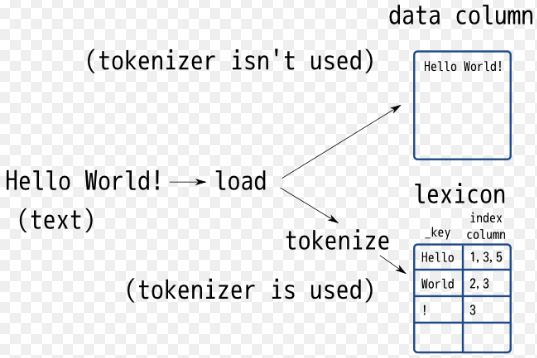
\includegraphics[width=1\textwidth]{figures/huda/chapter7/1.JPG}}
	\caption{Tokenizer}
	\label{c7_1}
\end{figure}
\item Jelaskan apa itu Deep Learning.
\subitem Deep Learning merupakan cabang dari Machine Learning atau bagian keluarga yang lebih luas dari method machine learning berdasarkan pada representasi data pembelajaran dan memiliki konsep serupa, tapi dilakukan dengan metode yang lebih cerdas. Deep Learning menggunakan Deep Neural Network dalam menyelesaikan suatu masalah yang terjadi pada Machine Learning.
\item Jelaskan apa itu Deep Neural dan bedanya dengan Deep Learning.
\begin{itemize}
\item Deep Neural Network atau DNN merupakan algoritma yang berbasis neural network yang digunakan untuk mengambil keputusan.
\item Yang membedakan Deep Learning dengan  Deep Neural Network (DNN) adalah DNN merupakan algoritma yang digunakan pada Deep Learning, sedangkan Deep Learning merupakan model yang menggunakan algoritma DNN.
\end{itemize}
\end{enumerate}